\documentclass{standalone}
\usepackage{tikz-network}

\begin{document}
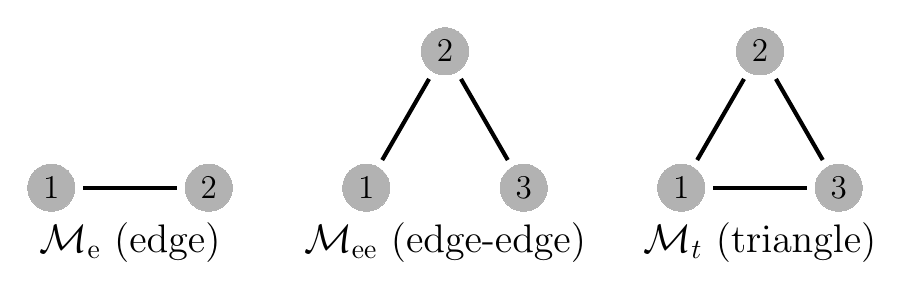
\begin{tikzpicture}

\SetVertexStyle[LineWidth=0, FillColor=black!30!white, LineColor=black!30!white, OuterSep=3, TextFont=\large]
\SetEdgeStyle[Color=black]
\SetTextStyle[TextFont=\Large]

\Vertex[label=1]{Me_1}
\Vertex[x=2,label=2]{Me_2}
\Edge[](Me_1)(Me_2)
\Text[x=1,y=-0.7]{$\mathcal{M}_\textrm{e}$ (edge)}

\Vertex[x=4,label=1]{Mee_1}
\Vertex[x=5,y=1.732,label=2]{Mee_2}
\Vertex[x=6,label=3]{Mee_3}
\Edge[](Mee_1)(Mee_2)
\Edge[](Mee_2)(Mee_3)
\Text[x=5,y=-0.7]{$\mathcal{M}_\textrm{ee}$ (edge-edge)}
 
\Vertex[x=8,label=1]{Mtr_1}
\Vertex[x=9,y=1.732,label=2]{Mtr_2}
\Vertex[x=10,label=3]{Mtr_3}
\Edge[](Mtr_1)(Mtr_2)
\Edge[](Mtr_2)(Mtr_3)
\Edge[](Mtr_3)(Mtr_1)
\Text[x=9,y=-0.7]{$\mathcal{M}_t$ (triangle)}
 
\end{tikzpicture}
\end{document}